% !TeX program = xelatex
% Build: latexmk -interaction=nonstopmode -halt-on-error paper.tex
% The iftex font branches also support pdfLaTeX and LuaLaTeX.
% Optional reviewer layout: define \ReviewMode before inputting this file.
\ifdefined\ReviewMode
\documentclass[12pt,letterpaper]{article}
\else
\documentclass[12pt,letterpaper]{article}
\fi
\usepackage[margin=1in,headheight=15pt]{geometry}
\usepackage{iftex}
\usepackage{amsmath,amsthm}
\ifPDFTeX
  \usepackage[T1]{fontenc}
  \usepackage[utf8]{inputenc}
  \usepackage{newtxtext,newtxmath}
  \usepackage[scaled=0.95]{helvet}
  \usepackage{inconsolata}
\else
  \usepackage{fontspec}
  \IfFileExists{STIXTwoText-Regular.otf}{
    \setmainfont{STIXTwoText-Regular.otf}[BoldFont=STIXTwoText-Bold.otf,ItalicFont=STIXTwoText-Italic.otf,BoldItalicFont=STIXTwoText-BoldItalic.otf]
  }{
    \setmainfont{lmroman10-regular.otf}[BoldFont=lmroman10-bold.otf,ItalicFont=lmroman10-italic.otf,BoldItalicFont=lmroman10-bolditalic.otf]
  }
  \setsansfont{lmsans10-regular.otf}[BoldFont=lmsans10-bold.otf,ItalicFont=lmsans10-oblique.otf]
  \setmonofont[Scale=0.88]{lmmono10-regular.otf}
  \usepackage{unicode-math}
  \IfFileExists{STIXTwoMath-Regular.otf}{\setmathfont{STIXTwoMath-Regular.otf}}{\setmathfont{latinmodern-math.otf}}
\fi
\usepackage{booktabs,tabularx,longtable,array,graphicx}
\usepackage{xurl}\usepackage{microtype,setspace,enumitem,float,placeins,caption,fancyhdr,xcolor}
\usepackage[round,authoryear]{natbib}
\newcommand{\QFullGrowth}{8.82}
\newcommand{\QFullDrawdown}{81.08}
\newcommand{\QFullWater}{175}
\newcommand{\QLaterGrowth}{19.44}
\newcommand{\QLaterDrawdown}{32.58}
\newcommand{\QLaterWater}{24}
\newcommand{\RFullGrowth}{9.17}
\newcommand{\RFullDrawdown}{17.23}
\newcommand{\RFullWater}{43}
\newcommand{\RLaterGrowth}{13.09}
\newcommand{\RLaterDrawdown}{13.91}
\newcommand{\RLaterWater}{19}
\newcommand{\MFullGrowth}{11.07}
\newcommand{\MFullDrawdown}{27.94}
\newcommand{\MFullWater}{48}
\newcommand{\MLaterGrowth}{14.83}
\newcommand{\MLaterDrawdown}{27.94}
\newcommand{\MLaterWater}{29}

\usepackage[unicode,hidelinks,pdfauthor={Yudian Pan},pdftitle={Regime-Aware Nasdaq Allocation: Growth, Drawdowns, and Recovery}]{hyperref}
\usepackage[capitalise,noabbrev]{cleveref}
\ifdefined\ReviewMode\doublespacing\else\setstretch{1.08}\fi
\setlength{\parindent}{1.3em}
\setlength{\parskip}{4pt}
\setlength{\emergencystretch}{3em}
\widowpenalty=10000
\clubpenalty=10000
\setlength{\bibsep}{5pt}
\renewcommand{\topfraction}{0.9}
\renewcommand{\bottomfraction}{0.85}
\renewcommand{\textfraction}{0.08}
\renewcommand{\floatpagefraction}{0.75}
\captionsetup{font=small,labelfont=bf,justification=raggedright,singlelinecheck=false}
\pagestyle{fancy}\fancyhf{}\fancyhead[L]{\footnotesize REGIME-AWARE NASDAQ ALLOCATION}\fancyhead[R]{}\fancyfoot[C]{\thepage}
\renewcommand{\headrulewidth}{0.3pt}
\newcommand{\E}{\mathbb E}\newcommand{\R}{\mathbb R}\newcommand{\1}{\mathbf 1}
\newcommand{\QQQ}{\text{QQQ}}\newcommand{\CAGR}{\operatorname{CAGR}}
\newcommand{\Note}[1]{\par\vspace{3pt}{\footnotesize\noindent\emph{Notes:} #1\par}}
\newcolumntype{Y}{>{\raggedright\arraybackslash}X}
\newcommand{\ResearchTable}[4]{\begin{table}[htbp]\centering\caption{#1}\label{#2}{\small\input{tables/#3}}\Note{#4}\end{table}}
\title{\vspace{-1.3cm}\textbf{Regime-Aware Nasdaq Allocation:\\Growth, Drawdowns, and Recovery}}
\ifdefined\AnonymousMode\author{Anonymous manuscript}\hypersetup{pdfauthor={}}\else\author{Yudian Pan}\fi
\date{October 13, 2026\\\small Return observations through September 2026}
\begin{document}
\maketitle\thispagestyle{empty}
\begin{abstract}
We examine whether monthly state-sensitive allocation improves the growth, drawdown, and recovery trade-off of a Nasdaq-oriented portfolio. A transparent rule and a constrained optimizer allocate across equities, bonds, gold, and reserves. Over January 2000--September 2026, their maximum month-end drawdowns are 17.23\% and 27.94\%, compared with 81.08\% for Nasdaq buy-and-hold. Full-history protection exceeds that of constant portfolios with matched average holdings or realized volatility. The growth advantage is unstable across investment starting dates, however. During 2016--2025, both methods trail buy-and-hold, and a simple ten-month trend rule produces higher growth and smaller drawdowns than either. A loss classifier fails to improve on event frequency; authentic historical macroeconomic vintages add little forecast accuracy. Paired resampling does not establish positive growth outperformance. The results support a historical downside-control interpretation while exposing the opportunity cost and model dependence of additional complexity. Calculations use frozen monthly proxies: a daily-bar follow-up bounds one early-price discrepancy and tests next-session execution. Larger daily drawdowns and changed timing comparisons preclude interpreting monthly results as validated attainable returns.
\end{abstract}
\noindent{\footnotesize AI disclosure: ChatGPT assisted with research design, literature search, code, analysis and writing. Full disclosure appears in the declarations.}\par
\noindent\textbf{Keywords:} asset allocation; Nasdaq-100; volatility management; drawdown; recovery; real-time data.\\
\textbf{JEL classifications:} G11, G17, C53, C61.

\section{Introduction}
An investor can recover a previous portfolio high while still lagging its purchasing power or a passive equity benchmark. These outcomes distinguish loss control from investment success. A Nasdaq-oriented allocation makes the distinction visible because its history includes both prolonged declines and extended periods of rapid equity appreciation.

This paper asks how observable market states and cost-aware allocation change that trade-off. Rule R combines equity trend indicators, defensive-asset filters, and state-dependent volatility budgets. Optimizer M maximizes a regularized forecast under risk, concentration, and trading-cost constraints. Both invest monthly without leverage across Nasdaq-100 equities, broad U.S. equities, aggregate bonds, gold, and reserves. The contribution is an empirical comparison of established methods, with recovery and information timing treated as separate outcomes and constraints.

The analysis distinguishes dynamic allocation from holding less equity. Constant portfolios match average holdings or validation-period volatility, and a ten-month trend rule supplies a simpler active comparator. Rolling investment starts assess dependence on the dot-com starting point. Forecast evaluation, macroeconomic vintages, and independent numerical accounting provide additional tests of the proposed interpretation. The unfavorable comparisons are central: the complex methods' full-history protection does not establish a stable growth advantage or a unique benefit from their state representation.

The study is a retrospective chronological evaluation. Earlier development already inspected the historical periods, including the later evaluation window. The current analysis retains the inherited R and M specifications and reports additional controls without choosing a replacement winner. All performance claims remain conditional on the documented monthly inputs and cost convention.

\section{Related literature}
\citet{devanathan2026} study monthly unlevered stock, bond, gold, and cash portfolios over 2006--2026. They compare fixed allocations, volatility control, and convex optimization using simple and macroeconomic forecasts. Their study motivates the present Nasdaq-oriented extension. The asset universe, historical proxies, risk budgets, and accounting differ, so the present calculations are a separate implementation rather than a replication of their reported portfolios. \citet{boyd2024} provide the broader cost-aware portfolio-construction framework.

Earlier research provides several models of state-dependent allocation. \citet{guidolin2007} study regime-switching asset-return distributions; \citet{nystrup2019} combine state forecasts with multi-period portfolio decisions and drawdown control. Here, a deterministic indicator score defines operational allocation states. Moving-average timing also has a long history in tactical allocation \citep{faber2007}. The simple trend comparator tests whether a more elaborate state rule adds useful performance in this particular universe.

The evidence on volatility management depends on design. \citet{moreira2017} report favorable risk-adjusted performance, while \citet{cederburg2020} find that implementable out-of-sample benefits are less reliable across a wider strategy set. \citet{bessler2021} likewise show that allocation rankings vary across investment horizons and economic conditions in a different factor-and-sector universe. These results motivate comparisons across periods and baselines, without treating their samples as independent replications of the present study.

Selection and dependence constrain inference. \citet{bailey2017} analyze backtest overfitting, and \citet{lo2002} show why Sharpe-ratio inference depends on the return process. This study reports paired block resampling and serial-dependence diagnostics. Their scope is the stated model family and observed history; unrecorded earlier specification searches remain outside the statistical correction.

\section{Data, proxies, and the information clock}
\subsection{Asset universe and sample construction}
The evaluation sample contains 321 monthly returns from January 2000 through September 2026. Nine preceding monthly returns, April--December 1999, are used for initialization. The starting wealth date is December 31, 1999. All base-case returns are in U.S. dollars and reinvest distributions. The model has no external cash flows or personal taxes.

\begin{table}[htbp]\centering
\caption{Research exposures and historical instruments}\label{tab:data}
\small\begin{tabularx}{\textwidth}{@{}>{\raggedright\arraybackslash}p{2.6cm}>{\raggedright\arraybackslash}p{2.3cm}Y@{}}\toprule
Exposure & Main instrument & Earlier observations and limitations\\\midrule
Nasdaq-100 & QQQ & Actual ETF history from 1999; used as a proxy for a prospective QQQM holding, not as an identical fee history.\\
Broad U.S. equity & VTI & VTSMX before the VTI splice in 2001; mutual-fund and ETF histories are not identical trading vehicles.\\
Aggregate bonds & BND & VBMFX before the BND splice in 2007; includes non-Treasury risks and is not cash.\\
Gold & GLD & Indicative spot prices with an assumed custody charge before the 2004 splice; used as a proxy for prospective GLDM exposure.\\
Short reserve & Bill-rate proxy & Previous-month TB3MS divided by 1,200, less 9 basis points per year; not an observed SGOV total-return series.\\
Secondary benchmark & SPY & Actual S\&P 500 ETF total-return proxy.\\\bottomrule
\end{tabularx}
\Note{Exact monthly mappings and the frozen observations are supplied in \texttt{raw/}. An instrument's modern ticker does not imply that it existed throughout the sample.}
\end{table}

The inherited prices originate from secondary-vendor adjusted-price tables \citep{digrin2026}; the early gold segment uses an indicative spot source \citep{metalflow2026}. A documented 1999 warm-up supplements the evaluation history. Most price observations have only two decimal places. Rounding can matter materially for low-price bond-fund histories. These are not independently audited exchange or custodian NAV records. Appendix~\ref{app:external} reports 39 independent aggregate issuer and SEC checkpoints. Modern comparisons differ by up to 13.72 basis points; an early QQQ market-return comparison differs by 77.31 basis points. NAV comparisons involve a different return basis. A daily-price audit narrows the early discrepancy, and fixed return perturbations and a complete QQQ source substitution preserve the central interpretation (Appendix~\ref{app:external}). No aggregate adjustment is imposed on the frozen observations.

The QQQ and GLD histories already reflect their historical fund-level expenses. We do not subtract today's QQQM or GLDM fee again. Conversely, the cash and pre-fund gold series include explicit modeling assumptions rather than observed ETF expenses. The share-class and tax consequences of replacing these instruments in a real account are not estimated.

\subsection{Decision and observation timing}
Let $t$ denote a completed month-end and $r_{i,t+1}$ the subsequent monthly return. Indicators and forecasts use observations through $t$ and determine weights applied to $r_{i,t+1}$. The inherited engine follows this information order but assumes a month-boundary fill. A separate daily-bar experiment freezes each target at the completed signal close and trades at the next observed opening bar in the 2012--2026 ETF era. The close and next-open branches use the same daily panel, including BIL reserves; their results are not spliced into the earlier monthly proxy history.

The initial covariance estimate uses only nine observations. Where a full lookback is unavailable, the implementation uses the available history; in particular, the early moving-average slope compares expanding rather than uniformly full ten-month averages. This initialization is disclosed rather than disguised as a long pre-2000 training sample.

For macroeconomic predictors, we acquire the Philadelphia Fed's official monthly vintage matrices for seasonally adjusted CPI and manufacturing production \citep{phillypcpi2026,phillyipm2026}. At signal month $t$, the feature constructor admits a vintage dated no later than $t-1$ and uses reference observation $t-2$. This extra vintage-month lag conservatively accommodates within-month release timing. Each growth ratio uses exact lags within one vintage. Appendix~\ref{app:macro} specifies missingness, fallback rules, and the matched latest-vintage comparison.

The production definitions require particular care. The Philadelphia Fed's IPM history uses the Standard Industrial Classification (SIC) manufacturing series, whereas the inherited FRED IPMAN observations use the North American Industry Classification System (NAICS). Their differences combine definition and revision effects \citep{phillyipmdoc,fredipman}. The new comparison uses SIC on both sides to isolate the effect of vintage information within that definition. The inherited macro branch remains a separately labeled exploratory output.

Latest-vintage CPI serves only to evaluate ex-post purchasing power. Its overlapping nonmissing levels agree exactly with the inherited CPI observations. The real-performance sample ends in December 2025; the absent October 2025 observation remains missing, with elapsed calendar time preserved. The reserve sleeve uses a lagged bill-rate approximation, not an observed bill-fund total return or a complete historical release-vintage record.

\section{Portfolio methods}
\subsection{R: transparent state-dependent risk allocation}\label{sec:R}
For each equity exposure $j\in\{Q,U\}$, define a total-return price index $P_{j,t}$ and three binary indicators:
\begin{align}
T_{j,t}&=\1\{P_{j,t}>MA_{10,j,t}\},\\
A_{j,t}&=\1\{R^{(6)}_{j,t}>R^{(6)}_{c,t}\},\\
S_{j,t}&=\1\{MA_{10,j,t}>MA_{10,j,t-3}\}.
\end{align}
Here $R^{(6)}$ is the compounded return over the same trailing six-month window, including the reserve comparison. The state score is
\begin{equation}
z_t=\sum_{j\in\{Q,U\}}(T_{j,t}+A_{j,t}+S_{j,t}).\label{eq:score}
\end{equation}
Scores of 5--6 designate risk-on, 2--4 transition, and 0--1 defensive. These are operational labels. Overlapping equity holdings and similar lookbacks make the six indicators dependent; a score of five is not five independent pieces of evidence or an 83\% probability of a positive return.

\begin{table}[htbp]\centering
\caption{R allocation templates before asset filters and risk scaling}\label{tab:templates}
\small\begin{tabular}{@{}lrrrrrr@{}}\toprule
State & Nasdaq & U.S. & Bonds & Gold & Reserve & Risk budget\\\midrule
Risk-on & 65\% & 20\% & 10\% & 5\% & 0\% & 15\%\\
Transition & 30\% & 15\% & 20\% & 15\% & 20\% & 12\%\\
Defensive & 10\% & 0\% & 35\% & 25\% & 30\% & 8\%\\\bottomrule
\end{tabular}
\Note{Templates are stipulated policy assumptions, not optimized ex post weights. Risk budgets refer to estimated annualized volatility, not realized loss limits.}
\end{table}

Bonds and gold independently must satisfy both their own ten-month trend test and six-month return test relative to reserves. A failed sleeve is moved to reserves rather than reassigned to another declining risky asset. Let $v_t$ be the resulting four-dimensional risky weight vector, and let $\widehat\Sigma_t$ be the monthly covariance estimate. Risk scaling gives
\begin{align}
a_t&=\min\left\{1,\frac{\sigma_{s_t}}{\sqrt{12v_t^\top\widehat\Sigma_t v_t}}\right\},\\
w_t&=a_tv_t,\qquad w_{c,t}=1-\1^\top w_t.\label{eq:scaling}
\end{align}
The rule allocates the full portfolio between risky assets and reserves. Defensive templates retain limited equity exposure, and the estimated volatility budget determines the final scale.

\subsection{M: simple cost-aware constrained optimization}\label{sec:M}
M uses the preceding 36 months of excess returns when available, with a 12-month exponential half-life, and shrinks the estimated monthly mean halfway toward a stipulated prior:
\begin{equation}
\widehat\mu_t=\operatorname{clip}\left(0.5\,\operatorname{EWMA}_{12}(r-r_c)_t+0.5\mu_0,-0.025,0.025\right),
\end{equation}
where $12\mu_0=(0.06,0.045,0.01,0.005)^\top$. The monthly clipping limits and stipulated priors regularize the forecast.

Let $\widetilde w=(w,1-\1^\top w)$ contain reserve weight and let $\widetilde w_t^{-}$ denote drifted pre-trade weights. The general optimization family solves
\begin{equation}
\max_w\quad \widehat\mu_t^\top w-\kappa\|U_tw\|_2-c\|\widetilde w-\widetilde w_t^{-}\|_1,\label{eq:opt}
\end{equation}
subject to
\begin{align}
w&\ge0,\qquad \1^\top w\le1,\qquad \sqrt{12w^\top\widehat\Sigma_tw}\le\sigma_t,\\
w_Q&\le0.85,\quad w_U\le0.60,\quad w_B\le0.60,\quad w_G\le0.35,\\
w_Q+w_U&\le e_t,\\
\|w-(\1^\top w)b\|_1&\le\1^\top w,\qquad b=(0.50,0.20,0.20,0.10)^\top.\label{eq:relative}
\end{align}
M sets $\kappa=0$, $\sigma_t=15\%$, and $e_t=95\%$. The relative-weight constraint limits deviation from a reference allocation conditional on the total risky investment. It does not require maintaining a fixed amount of risk exposure.

For the robust variant, $U_t$ is a diagonal scale for mean-estimation uncertainty. If the true mean lies in an ellipsoid $\{\widehat\mu_t+U_tu:\|u\|_2\le\kappa\}$, its minimum portfolio mean is $\widehat\mu_t^\top w-\kappa\|U_t^\top w\|_2$. Because $U_t$ is diagonal, this gives the penalty in \cref{eq:opt}. The uncertainty set remains an estimated modeling device, not a confidence guarantee.

The feasible set is convex and the objective is concave. The implementation uses an absolute-cost epigraph and SLSQP with analytic gradients, followed by a feasibility check. Failed candidates fall back to reserves. For M, a separate HiGHS linear program bounds the objective from above using outer approximations of the quadratic risk constraint; feasible candidates supply lower bounds. All 321 monthly problems meet the stated numerical tolerance (Appendix~\ref{app:solver-bounds}). This check establishes solution quality conditional on the fitted estimates.

\subsection{Additional variants and forecasting experiment}
MR replaces the simple mean with a regularized regression forecast. Training labels are three-month forward excess compound returns divided by three; all three months must have matured at the signal date. At least 60 valid labels are required, with at most about 120 recent labels, training-only standardization, and a ridge penalty of ten. Forecasts are shrunk toward the same prior and clipped. Appendix~\ref{app:forecast} provides the implementable details.

RM combines the regression forecast with $\kappa=0.25$, the three state-dependent volatility budgets, and equity caps of 95\%, 65\%, and 25\%. PM instead uses a logistic forecast $p_t$ to set $\sigma_t=15\%(1-0.5p_t)$ and $e_t=95\%-0.7p_t$. The macro extensions add three CPI and manufacturing features using either conservative as-of or latest-vintage observations. The extensions isolate the contribution of each additional modeling choice.

The classifier predicts the specific event
\begin{equation}
Y_t=\1\left\{\prod_{k=1}^{3}(1+r_{Q,t+k})-1\le-0.10\right\}.\label{eq:label}
\end{equation}
This event targets a specific three-month equity loss. A logistic model with four predetermined price features and an $L_2$ penalty is evaluated against a smoothed training-window event frequency. Forecast accuracy is evaluated separately from the resulting investment performance across all eligible dates.

\section{Trading, costs, and evaluation}
\subsection{Self-financing accounting}
Let $h_i^{-}$ denote pre-trade dollar holdings and $V^{-}$ their sum. A rebalance finds post-cost wealth $V^{+}$ and holdings $h_i^{+}=V^{+}\widetilde w_i$ satisfying
\begin{equation}
V^{+}=V^{-}-\sum_i c_i|h_i^{+}-h_i^{-}|-fN_{\mathrm{orders}}-C_{\mathrm{FX}}.\label{eq:account}
\end{equation}
Subsequent wealth is $V_{t+1}^{-}=\sum_i h_i^{+}(1+r_{i,t+1})$. The base engine solves the self-consistency relation by fixed-point iteration; a second holdings implementation uses bisection. Initial deployment is charged once as purchases from external cash. The reserve is a modeled investment sleeve, so switches to and from it are included in later turnover.

The base case sets $c_i=10$ basis points per absolute dollar bought or sold. A complete switch from one asset to another can therefore incur both sale and purchase charges. Fixed dollar fees and initial/final currency conversion are separate scenarios. Base terminal wealth remains invested; final liquidation is not silently charged to active strategies alone. Fund-level costs already embodied in observed returns are not deducted again.

A two-percentage-point no-trade band applies only when the state has not changed and the current portfolio still meets the estimated risk and equity-cap checks. Price drift is retained between trades. Minimum-ticket fees, trading spreads, taxes, order fills, and whole-share constraints are distinct implementation issues; a monthly decision frequency does not imply only twelve orders per year.

\subsection{Performance and recovery metrics}
For $N$ months, base CAGR is $(V_N/V_0)^{12/N}-1$. The conventional reported volatility is $\sqrt{12}\operatorname{Std}(r_p)$ and the reported Sharpe ratio is $\sqrt{12}\operatorname{Mean}(r_p-r_c)/\operatorname{Std}(r_p-r_c)$. These are standardized monthly-sample summaries, not exact time-aggregation identities under serial dependence. Appendix~\ref{app:inference} provides a separate finite-horizon diagnostic motivated by \citet{lo2002}.

Define month-end drawdown as
\begin{equation}
D_t=1-\frac{V_t}{\max_{s\le t}V_s}.
\end{equation}
Maximum drawdown is the greatest observed $D_t$. Time under water starts at a prior wealth high and ends when that high is regained. Durations count elapsed monthly steps through the recovery endpoint. An unfinished episode is right-censored. This measure differs from trough-to-recovery time. The latter ignores how long the decline itself took.

Relative downside is also evaluated over common Nasdaq-high-to-subsequent-month windows. We compare both investments over the same dates, rather than subtracting maximum drawdowns attained on different dates. These common-date losses measure benchmark-relative downside separately from each portfolio's own maximum drawdown.

Real wealth is $V_t^{\mathrm{real}}=V_t\,\mathrm{CPI}_0/\mathrm{CPI}_t$. Nominal recovery need not restore purchasing power. The calculation preserves unitized wealth without external contributions.

\section{Research design and selection discipline}
The study uses 2000--2009 as development history, 2010--2015 for one explicit method-selection exercise, 2016--2025 for the historical chronological audit, and January--September 2026 as a supplement. A 2012-onward comparison reduces reliance on pre-inception asset proxies. All dates and candidates remain visible.

Validation eligibility requires observed maximum drawdown no larger than 30\%, annual two-way turnover no larger than six times wealth, and longest water duration no longer than 48 months. Among eligible methods the stipulated score is $\log(1+\CAGR)-\tfrac12\sigma^2$. This is a preference score, not a universal welfare criterion. It selects M; its name is then retained for the later audit regardless of its subsequent rank.

Each subperiod metric table starts with fresh cash and charges initial deployment, while estimators retain legitimately earlier observations. The no-trade state is reinitialized. In contrast, crisis-window returns and the serial-correlation diagnostic slice the continuous full-history portfolio. These accounting conventions are intentionally distinguished; the later audit is not presented as a single uninterrupted investor account that began in 2000.

Parameter choices were locally frozen for the preceding computational round, after earlier market histories had already been inspected. The 2026 data supplement is not an untouched prospective test. Sensitivity analysis characterizes nearby assumptions; it is not permission to replace a prespecified method with whichever variant wins after inspection.

\subsection{Simple controls and attribution}
For each active policy, the first constant control holds its arithmetic mean monthly post-trade weights. The second holds a fixed QQQ/reserve mixture whose realized volatility matches the active policy during calibration. For the 2016--2025 evaluation, both controls freeze their weights using only 2010--2015 observations, then rebalance monthly with the same cost accounting. Evaluation-period risk and exposure can differ from their calibration targets. Separate full-history matches use hindsight and serve only as descriptive attribution checks.

The trend comparator holds QQQ when its observed total-return index exceeds its trailing ten-month average, and reserves otherwise. It uses the same monthly clock and ten-basis-point trading charge. Its lookback is fixed before this revision's new comparisons; the historical sample remains previously observed. No additional predictor or asset is introduced.

\section{Empirical results}
\subsection{Protection across the full history, slower growth later}
\ResearchTable{Full-history performance, January 2000--September 2026}{tab:full}{full.tex}{321 monthly returns. All methods use modeled costs and the same frozen dollar-return inputs. MDD is the positive magnitude of maximum month-end drawdown. Water is the longest elapsed time from a previous high through recovery, in months. Static 70/20/10 denotes Nasdaq/bonds/gold.}

R earned \RFullGrowth\% annually with a \RFullDrawdown\% maximum drawdown; M earned \MFullGrowth\% with a \MFullDrawdown\% drawdown. QQQ earned \QFullGrowth\% with a \QFullDrawdown\% drawdown. The wealth and drawdown paths show how avoiding part of the prolonged early losses changed subsequent compounding (Figures~\ref{fig:wealth} and~\ref{fig:drawdown}). R's lower loss depth came with lower growth than M and higher trading intensity.

\ResearchTable{Later historical evaluation, January 2016--December 2025}{tab:later}{later.tex}{120 months; fresh initial cash positions, with preceding observations available to estimators. This period was inspected in earlier development. Trend denotes the fixed ten-month QQQ/reserve rule.}

The later period favored sustained equity participation. R and M earned \RLaterGrowth\% and \MLaterGrowth\%, against QQQ's \QLaterGrowth\%. R reduced the longest nominal water period to \RLaterWater\ months; M's \MLaterWater\ months exceeded QQQ's \QLaterWater\ months. Smaller maximum drawdown therefore did not guarantee faster recovery for M.

The simple trend rule earned 16.83\% with a 13.06\% maximum drawdown and 15 months under water. It exceeded both R and M on these three measures. R retained lower realized volatility, 10.87\% versus the trend rule's 14.17\%. Thus the comparison supports different risk preferences, but provides no general performance justification for the additional state-rule complexity in the later window.

\begin{figure}[htbp]\centering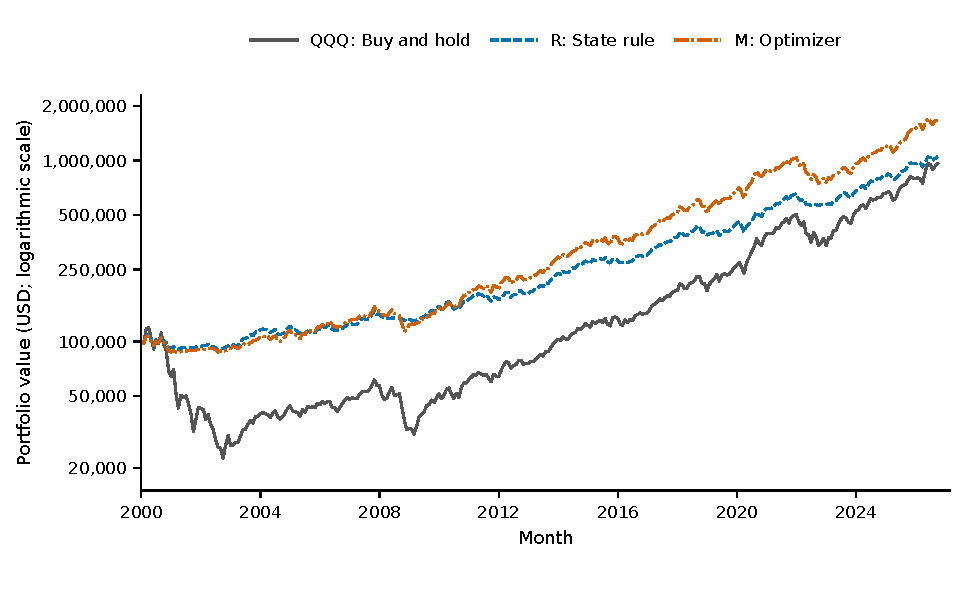
\includegraphics[width=165mm]{figures/wealth.pdf}
\caption{Wealth from \$100,000 over January 2000--September 2026. The logarithmic axis shows all 321 modeled monthly returns for QQQ, R, and M, plus the initial valuation. Straight segments connect observations; they do not represent intramonth prices. Source data reproduce each plotted value.}\label{fig:wealth}\end{figure}
\begin{figure}[htbp]\centering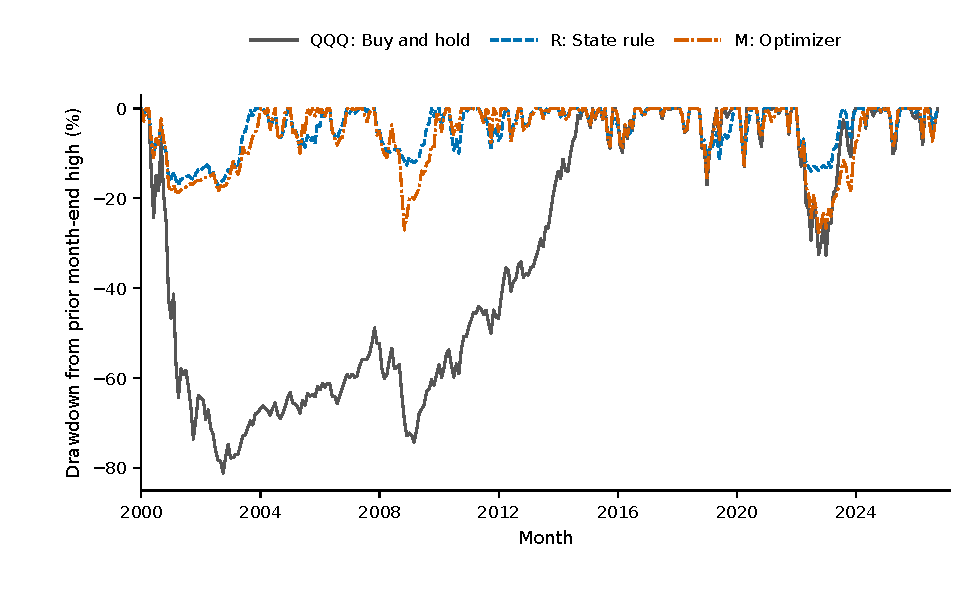
\includegraphics[width=165mm]{figures/drawdown.pdf}
\caption{Losses from previous month-end wealth highs on the same full-history paths. Each curve includes all 322 valuations. These realized monthly paths have no sampling error bars; they omit intramonth drawdowns and next-session execution effects.}\label{fig:drawdown}\end{figure}

\subsection{How much comes from lower exposure?}
\ResearchTable{Constant controls calibrated in 2010--2015, evaluated in 2016--2025}{tab:matched}{matched.tex}{Mean-holdings controls fix each active policy's average five-asset weights. Volatility-match controls fix QQQ/reserve weights that match calibration-period volatility. Equity is average realized QQQ plus broad-equity weight during evaluation. Controls rebalance monthly; their evaluation risk need not equal that of the active policy.}

In the full-history hindsight diagnostic, R's mean-holdings control had a 52.79\% maximum drawdown, compared with R's 17.23\%. M's control had a 59.86\% drawdown, compared with M's 27.94\%. The controls hold the same average asset vector, so lower average equity exposure alone does not explain the observed full-history protection. Volatility-matched QQQ/reserve portfolios also suffered larger drawdowns, 46.53\% and 58.10\%, respectively.

The validation-frozen controls reveal the later growth cost (Table~\ref{tab:matched}). Both active policies trailed their mean-holdings and volatility-match controls in CAGR. R retained a smaller drawdown than either of its controls. M's drawdown was slightly smaller than its mean-holdings control but slightly larger than its volatility-match control. These comparisons identify a path-dependent downside benefit, not a stable improvement in every performance dimension.

A sequential component analysis gives the same qualified interpretation. Adding volatility scaling to R's fixed risk-on template reduced full-history drawdown from 67.34\% to 39.63\%. Adding states reduced it to 18.97\%; the defensive-asset filters reduced it to 17.23\%. The last step lowered growth from 9.81\% to 9.17\% and lengthened recovery from 41 to 43 months. Appendix~\ref{app:ablation} retains both periods and the order-dependent nature of this attribution.

\subsection{Crises and investment starting dates}
\ResearchTable{Cumulative crisis-window returns}{tab:crisis}{crisis.tex}{Slices of the continuous full-history portfolio. The 2000--2002 column compounds three calendar years; other columns cover one year. These are calendar-window returns rather than peak-to-trough losses.}

R and M reduced losses during the dot-com and 2008 windows, but participated less in the 2020 rebound. R began 2000 in its risk-on state; volatility scaling nevertheless limited initial equity exposure to about 57.9\%. Some protection therefore preceded a change in its state label. Its subsequent reversals and delayed re-entry remain in the recorded path.

Across all completed January-start ten-year windows, R beat QQQ's CAGR in 3 of 17 windows and M in 8 of 17. Both had smaller maximum drawdowns in all 17. The corresponding five-year counts were 7 of 22 and 8 of 22 for growth, and 22 of 22 for drawdown. Figure~\ref{fig:rolling} displays all ten-year growth differences. These overlapping windows describe start-date sensitivity; treating them as independent binomial trials would exaggerate precision.

\begin{figure}[htbp]\centering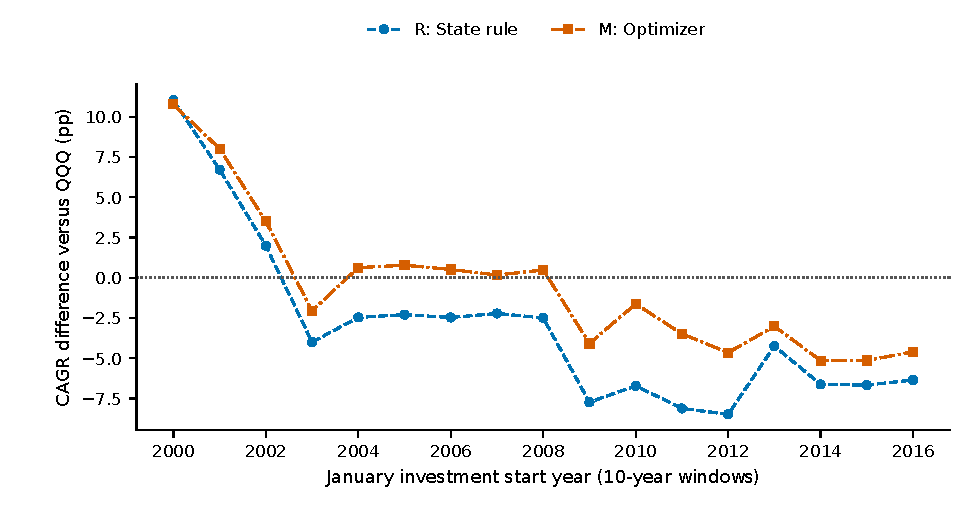
\includegraphics[width=165mm]{figures/rolling_growth.pdf}
\caption{Start-date dependence of annualized growth relative to QQQ. Each point is a fresh-start ten-year investment, with historical estimator warm-up retained. All 17 January starts from 2000 through 2016 end by December 2025. Differences are percentage points of CAGR, not differences in mean log returns. Windows overlap.}\label{fig:rolling}\end{figure}

\subsection{Forecasts and historical macroeconomic information}
The loss classifier did not improve on the contemporaneous smoothed event-frequency benchmark. Restricting every three-month outcome to 2016--2025 leaves 118 forecasts and seven event windows. Brier scores were 0.05871 for the model and 0.05855 for the baseline; AUC was 0.230. The original 120-origin window extended outcome follow-up into March 2026 and gave the same qualitative result (Appendix~\ref{app:macro}). Overlapping rare events limit inference; post-hoc reversal of the score would constitute a new model.

\ResearchTable{Macroeconomic vintage comparison under unchanged ridge rules}{tab:macro}{macro.tex}{Full history is January 2000--September 2026; later history is January 2016--December 2025. As-of and latest branches use the same SIC manufacturing definition and the same availability rule determined by the as-of branch. Water refers to the later period.}

The as-of macro extension increased full-history CAGR from price-only MR's 10.55\% to 10.91\%, but its later CAGR, 15.64\%, was close to MR's 15.56\%. The matched latest-vintage branch earned 15.65\% later. Portfolio returns alone do not establish predictive value. Over 118 outcome-bounded origins and four risky assets, the as-of extension reduced mean squared forecast error by only 0.28\%. A paired twelve-month-block interval for the loss difference crossed zero (Appendix~\ref{app:macro}). These results provide limited support for adding these macro features under this specification.

\subsection{Purchasing power and tail risk}
Latest official CPI extends QQQ's longest water period to 206 months, compared with 175 months nominally. R's longest real recovery was 86 months and M's 73, reversing their nominal ranking. Real CAGR over 2000--2025 was 6.36\% for R and 8.16\% for M, against 5.59\% for QQQ. Inflation raises the recovery threshold, so growth following the trough matters alongside the initial loss. The nominal and real endpoints differ explicitly; Appendix~\ref{app:additional} gives the complete real-performance table.

Full-history monthly expected shortfall at 95\%, measured as the mean loss among the worst 5\% of observed months, was 5.93\% for R, 7.72\% for M, and 15.09\% for QQQ. Annual two-way turnover was 2.35 times wealth for R and 0.95 for M. Lower tail loss therefore came with additional transactions. Common QQQ-high-to-subsequent-month windows also show that M could lose 10.10 percentage points more than QQQ over the same dates, despite its smaller own-path maximum drawdown.

\section{Uncertainty, costs, and interpretation}
Twenty thousand paired circular-block resamples evaluate annualized mean log-return differences using twelve-month blocks. Six dynamic comparisons across two windows form the inherited family of twelve tests. None establishes positive growth outperformance after Bonferroni correction. Six additional comparisons against the validation-frozen and trend controls likewise produce no adjusted positive-growth finding. The associated effect sizes and intervals remain visible in Appendix~\ref{app:inference}. Six- and 24-month block sensitivities do not support a stable positive-growth conclusion for R or M.

A second exercise reconstructs price paths, indicators, covariance estimates, forecasts, and portfolio decisions over 100 paired block-resampled asset histories. Growth-difference ranges cross zero for both policies. Drawdown reduction is more consistent, while some reconstructed histories have longer recovery than QQQ. The small replication count yields coarse tails. This exercise is descriptive process sensitivity; it neither repeats all historical model selection nor generates independent crises.

Costs and timing affect the economic interpretation. The 62-case sensitivity family varies risk budgets, covariance windows, costs, no-trade bands, information delay, and reserve remuneration. An additional month of signal delay raises M's maximum drawdown to 34.44\%. Removing realized reserve interest lowers full-history CAGR to 8.66\% for R and 10.82\% for M. A fixed-policy replay separates mechanical fee drag from cost-induced re-optimization; increasing fees monotonically lowers wealth when the trade policy is held fixed.

The central inference concerns conditional downside control. Dynamic allocation improved full-history losses beyond constant average-exposure controls, but simpler timing challenged the case for additional complexity. R and M also trade growth against volatility and recovery in different ways. An investor's preferred metric therefore determines the ranking. Figure~\ref{fig:frontier} illustrates this with the full static-allocation grid: its hindsight growth winner places 60\% in gold, above M's 35\% cap. A retrospective frontier under different constraints cannot identify an ex-ante optimal allocation.

\section{Limits and implications}
The daily follow-up changes the strength of several comparisons. For 2016--2025 at a ten-basis-point trading allowance, next-open R and M earn 12.88\% and 14.86\% annually, compared with 19.68\% for QQQ and 16.74\% for Trend10. R's maximum month-end drawdown is 13.53\%, below Trend10's 15.66\%: the simpler rule's three-metric superiority in the original monthly calculation does not survive this execution convention. R's daily-close drawdown is 25.61\%, substantially greater than its month-end measure. Monthly protection must not be presented as an intramonth loss limit. Appendix~\ref{app:external} reports the full matched experiment.

Three limits remain. First, a contemporaneous SEC close and daily dividend reconstruction constrain but do not fully identify the 2009 issuer discrepancy. A complete QQQ substitute and 26 fixed perturbations preserve the principal downside interpretation; unrelated mutual-fund and spot-gold errors are outside that bound. Second, opening bars and theoretical ex-date total-return units do not establish fill size, spreads, dividend payment-date cash availability, settlement, or whole-share feasibility. Third, prior inspection of the historical windows prevents prospective validation. A prospective evaluation requires a fixed protocol and subsequent observations.

The vintage reconstruction resolves a narrower problem. It supplies authentic monthly snapshots for the CPI and SIC production experiment, with conservative availability and explicit missingness. It does not reconstruct the legacy NAICS series or prove exact release-time availability for every source. Adding credit spreads or further indicators without a new hypothesis and fixed evaluation protocol would enlarge the search space without resolving the present forecasting weakness.

These qualifications align the interpretation with the volatility-management literature. The study documents protection in a concentrated equity setting across several different declines, while exposing the cost of reduced participation and the instability of relative growth. Its contribution lies in the joint assessment of growth, loss depth, recovery, simple controls, and information timing. Numerical optimality of the fitted M problem is useful for reproducibility, but remains separate from the quality of the return forecast.

\section{Conclusion}
Monthly risk-sensitive allocation reduced prolonged losses in the frozen 2000--2026 history, beyond what constant average-exposure controls achieved. That protection did not yield a stable growth advantage. The later period and rolling starts favored equity participation, and a simple trend rule outperformed both principal methods on growth, drawdown, and recovery in the frozen monthly 2016--2025 calculation. Its drawdown advantage over R does not survive the next-open follow-up. Failed loss prediction and small macroeconomic forecast gains further constrain the case for complexity. Bounded price sensitivities preserve that interpretation, while the observed daily-bar study exposes additional timing and valuation-frequency risk. This is a working-paper result, not certification of an executable investment strategy.

\clearpage
\bibliographystyle{plainnat}
\bibliography{references}
\clearpage
\appendix
\section{Estimator and solver specification}\label{app:forecast}
\subsection{Covariance and forecast details}
Monthly risky excess returns are $x_s=r_s-r_{c,s}\1$. For the most recent $n=\min(36,\text{available})$ observations, normalized exponential weights have half-life six months. The weighted covariance uses the denominator $\max(1-\sum_s a_s^2,0.1)$. It is then shrunk 25\% toward its diagonal and receives a $10^{-8}$ diagonal ridge. Base-case covariance uses at least the nine observed warm-up returns; alternative variance floors are separate sensitivity tests.

The simple mean uses the same observation window but a twelve-month half-life. Ridge forecasts use an intercept and 18 price features: for each risky asset, six- and twelve-month compounded returns, deviation from the ten-month mean, and the log ratio of recent three-month to twelve-month volatility; two additional features are the Nasdaq's trailing twelve-month drawdown and the annualized latest reserve return. Short histories use available observations. A minimum of 60 valid matured labels is required. Training weights have a sixty-month half-life; means and standard deviations are fitted inside the training window; feature standard deviations have a $10^{-4}$ floor.

For origins $s$ with $s+3\le t$, the target is
\begin{equation}
y_{i,s}=\frac{1}{3}\left[\prod_{k=1}^{3}(1+r_{i,s+k})-\prod_{k=1}^{3}(1+r_{c,s+k})\right].
\end{equation}
This arithmetic monthly-equivalent target is not a geometric excess-return identity. The normalized weighted least-squares objective has ridge penalty ten. The return prediction is shrunk 50\% toward the stipulated prior. Uncertainty scales use weighted residual root mean squares divided by an approximate effective sample-size factor, with a floor of 0.00025 per month. The heuristic does not create a correctly calibrated confidence region for the mean.

PM's logistic features are Nasdaq's trend deviation, six-month momentum, short/long volatility log ratio, and trailing drawdown. The intercept is unpenalized, the other coefficients have an $L_2$ penalty, and the benchmark probability is $(n_{\rm events}+1)/(n_{\rm labels}+2)$. The training features are standardized using training-only values. PM falls back to its standard risk budget before a fitted probability is available.

\subsection{Cost epigraph and no-trade behavior}
The solver introduces five variables $u_i$ satisfying $u\ge\widetilde w-\widetilde w^{-}$ and $u\ge-(\widetilde w-\widetilde w^{-})$. Its objective adds $c\sum_i u_i$. The relative $L_1$ constraint is represented by all sixteen sign combinations over four risky weights. The annualized quadratic risk constraint is evaluated explicitly.

SLSQP uses an iteration limit of 160 and an objective tolerance of $10^{-10}$. Failed or infeasible candidates are replaced by reserves. The no-trade risk check permits the stated numerical factor of $1.001$ above the budget.

\subsection{Independent objective bounds for M}\label{app:solver-bounds}
For M, the cost epigraph makes the objective linear in $(w,u)$; the only nonlinear constraint is the convex quadratic $q(w)=12w^\top\widehat\Sigma_tw\le\sigma^2$. At any point $x$, convexity gives
\begin{equation}
q(w)\ge q(x)+\nabla q(x)^\top(w-x).
\end{equation}
Consequently, each half-space
\begin{equation}
24x^\top\widehat\Sigma_tw\le\sigma^2+12x^\top\widehat\Sigma_tx
\end{equation}
contains the feasible risk set. Retaining the linear portfolio constraints and replacing the risk set with these half-spaces yields a linear-programming outer approximation. Its maximized objective is an upper bound, $U_t$, while the objective of a feasible SLSQP candidate is a lower bound, $L_t$. The gap $U_t-L_t$ bounds candidate suboptimality for the fitted problem.

The audit uses HiGHS for the outer problem, with primal and dual feasibility tolerances of $10^{-9}$. Initial cuts are placed at the feasible incumbent and at four axis points; additional cuts would be added at the LP solution if needed. It examines every monthly candidate, including months in which the no-trade band subsequently retains existing positions. All 321 problems satisfy the objective-gap tolerance $2\times10^{-8}$. The largest gap is approximately $6.1\times10^{-10}$ in monthly-return objective units; the maximum measured primal violation is $7.3\times10^{-15}$. These are floating-point numerical bounds, not exact-arithmetic proofs. They concern the estimated one-period objective, independently of its ability to predict realized returns.


\clearpage

\section{Additional performance and attribution}\label{app:additional}
\ResearchTable{All inherited variants in the later evaluation}{tab:variants}{variants.tex}{Fresh starts over 2016--2025. MR uses ridge forecasts; RM adds state risk budgets and uncertainty penalties; PM uses loss probabilities. Legacy macro uses revised NAICS production with backward missing-value fallback and remains exploratory. Static 50/20/20/10 denotes Nasdaq/U.S. equities/bonds/gold.}
\ResearchTable{Live-ETF-era sensitivity, January 2012--September 2026}{tab:2012}{etfera.tex}{ETF availability reduces reliance on pre-inception proxies. This remains a monthly-close model; reserves remain rate-based.}
\ResearchTable{Real purchasing-power performance, January 2000--December 2025}{tab:realall}{realall.tex}{Latest official seasonally adjusted CPI; the missing October 2025 valuation is omitted without interpolation. Durations preserve elapsed calendar months. All listed longest episodes have recovered by the relevant endpoint.}
\ResearchTable{Tail risk and trading intensity over the full history}{tab:downside}{downside.tex}{Sortino uses the modeled reserve return as the monthly threshold and the root mean square of negative excess returns, including zero contributions from other months. The conventional annualization is $\sqrt{12}$. Monthly ES averages the worst $\lceil0.05N\rceil$ months; it is an empirical summary, not a loss bound. Two-way turnover includes buys and sells.}
\ResearchTable{Investment-start sensitivity}{tab:rolling}{rolling.tex}{Every completed January-start window ending by December 2025. Growth gap is the CAGR difference in percentage points. Counts refer to overlapping windows and have no independent-trial interpretation.}

\subsection{Sequential component analysis}\label{app:ablation}
The fixed risk-on template holds $[0.65,0.20,0.10,0.05,0]$. Scale only applies the 15\% risk budget. States plus scale uses all three templates and budgets, and full R additionally applies the bond and gold filters. All variants use the same returns, covariance estimator, ten-basis-point charges, and two-percentage-point no-trade band. A separate holdings implementation reconstructs full R to within $10^{-9}$ in normalized wealth. The sequence defines the attribution order; interacting controls prevent a causal interpretation of individual differences.
\ResearchTable{R component analysis}{tab:ablation}{v4_ablation.tex}{Percent units for CAGR and MDD; Water is elapsed months. Full history ends in September 2026, and the later period spans 2016--2025. These diagnostic variants do not replace R.}

\begin{figure}[htbp]\centering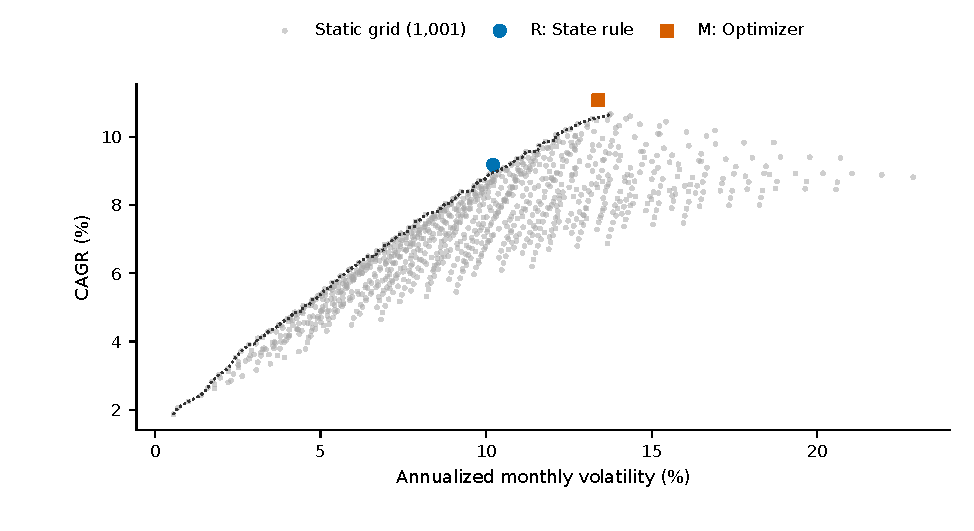
\includegraphics[width=165mm]{figures/hindsight_frontier.pdf}
\caption{Descriptive full-history growth--volatility frontier. Every point in the 1,001-portfolio, ten-percentage-point static simplex enters the plot. The dotted boundary connects grid allocations not dominated on CAGR and volatility. R and M provide dynamic references. Static allocations rebalance quarterly and can hold 100\% gold or reserves, unlike M's caps; the comparison uses full hindsight and different feasible sets. Recovery duration is a separate objective.}\label{fig:frontier}\end{figure}

\FloatBarrier
\section{Forecasts and macroeconomic vintages}\label{app:macro}
The official PCPI matrix contains 335 monthly vintages from November 1998 to September 2026; IPM contains 767 from November 1962 to September 2026. The script reads unmodified workbook XML and retains the source hashes. At each signal month $t$, it chooses the latest vintage $v\le t-1$ and reference observation $u=t-2$. The features are
\begin{align}
 \pi_t &= C_u^{(v)}/C_{u-12}^{(v)}-1,\\
 \Delta_6\pi_t &= \pi_t-\left(C_{u-6}^{(v)}/C_{u-18}^{(v)}-1\right),\\
 g_t &= I_u^{(v)}/I_{u-12}^{(v)}-1.
\end{align}
Each series uses its own admissible vintage; every numerator and denominator shares that series' vintage and index basis. Historical training features preserve the snapshot available at their own origin. The latest-vintage branch substitutes the September 2026 column while retaining the eligibility set determined solely by as-of information. It is a retrospective comparison, not an actionable forecast.

There are 318 complete macro feature sets among 321 actual allocation origins. Signals in November and December 2025 and June 2026 lack an exact required lag. Both branches use the price-only estimator at those origins; training excludes incomplete macro rows. An additional feature set for the next decision is retained separately. No missing value is interpolated, carried backward to a different lag, or replaced with a future vintage in the as-of branch.

The Philadelphia Fed's documentation identifies SIC manufacturing, including the classification-history issues surrounding the 2002 benchmark revision \citep{phillyipmdoc}. FRED IPMAN identifies NAICS manufacturing \citep{fredipman}. Comparing their index levels does not identify a pure vintage effect. The same-definition paired branches in Table~\ref{tab:macro} avoid that conflation. The three predictor features leave the ridge penalty, prior shrinkage, caps, costs, and risk budgets unchanged.

\ResearchTable{Outcome-horizon check for the loss classifier}{tab:classifier}{classifier.tex}{The first row reproduces the inherited origin-window definition and explicitly shows its 2026 follow-up. The second restricts outcomes to 2016--2025. The 118 origins run from December 2015 through September 2025. Event windows overlap; no probability threshold is tuned on either evaluation.}
\ResearchTable{Incremental macroeconomic forecast accuracy}{tab:macroforecasts}{macro_forecasts.tex}{MSE and differences are multiplied by $10^6$. Each branch contains 118 origins and 472 asset forecasts of three-month compound excess return divided by three. Monthly four-asset loss vectors remain paired in 9,999 circular-block draws of length 12. The 95\% percentile range is conditional on the realized fitted forecasts. This exploratory diagnostic was added after the portfolio specification and makes no multiplicity-adjusted discovery claim.}

\FloatBarrier
\section{Uncertainty and cost diagnostics}\label{app:inference}
For each comparison, $d_t=\log(1+r_{A,t})-\log(1+r_{B,t})$ and the statistic is $12\bar d$. Circular blocks preserve pairs, with 20,000 draws for the inherited twelve-comparison family. Centering the bootstrap statistic on its observed mean approximates the null for a one-sided positive-growth test. The six new control comparisons use 9,999 draws and their own Bonferroni family. These corrections concern the listed tests; they do not retrospectively preregister the study or correct unknown earlier searches.
\ResearchTable{Conditional paired log-growth inference versus QQQ}{tab:conditional}{conditional.tex}{Log-growth differences and ordinary percentile intervals are in percentage points per year. The adjusted one-sided $p$ values account for the complete inherited family of twelve tests. Familywise intervals and all candidates are retained in the CSV.}
\ResearchTable{Conditional inference versus the added simple controls, 2016--2025}{tab:matchedtests}{matched_tests.tex}{Units are annualized log-growth percentage points. Ordinary intervals describe effect uncertainty; adjusted one-sided $p$ values test positive active-policy growth across six comparisons. A negative ordinary interval is not a multiplicity-adjusted inferiority finding.}
\ResearchTable{Paired process-reconstruction sensitivity}{tab:boot}{boot.tex}{One hundred twelve-month-block histories, sampled jointly across the five assets including reserves. Each history reconstructs indicators and R/M decisions. Growth and drawdown differences are percentage points; Sharpe is unitless. Ranges are descriptive central 95\% ranges with coarse tails, not calibrated future intervals.}
\begin{figure}[htbp]\centering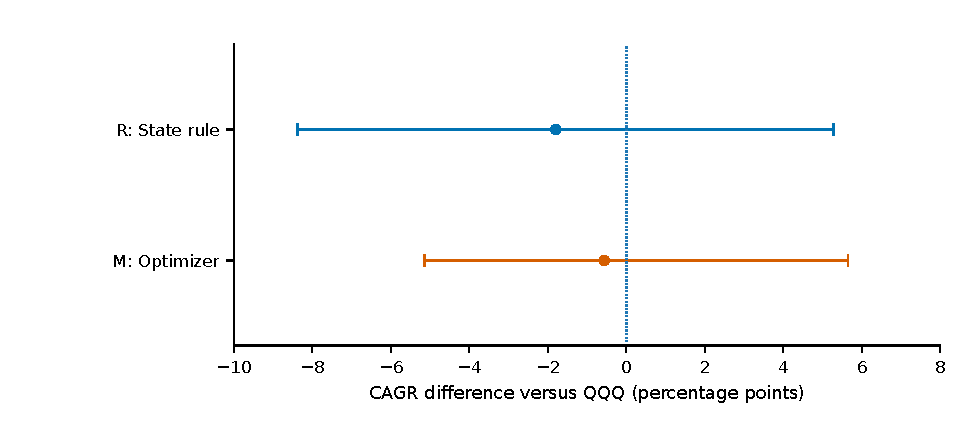
\includegraphics[width=165mm]{figures/bootstrap_growth.pdf}
\caption{Growth differences under process reconstruction. Points mark medians and bars mark empirical 2.5th and 97.5th percentiles across 100 paired histories per policy. Each policy and QQQ face the same resampled asset history. All 200 policy--replication observations enter the calculation. Model-family selection is held fixed.}\label{fig:bootstrap-growth}\end{figure}
\ResearchTable{Selected policy-recomputed sensitivities}{tab:sensitivity}{sensitivity.tex}{Full-history results. Each case recomputes the allocation, so changes in optimizer cost assumptions can also change decisions. An extra month of delay is an adverse timing scenario, not a substitute for next-session opening data.}
\ResearchTable{Fee drag with the base policy held fixed}{tab:replay}{replay.tex}{Base trade dates and post-trade target weights remain fixed; a bisection holdings ledger recomputes dollar costs at each fee level. This is a counterfactual cost decomposition.}

\subsection{Serial dependence}
For monthly excess return $x_t$, a separate stationary arithmetic-sum diagnostic estimates
\begin{equation}
 \widehat S_{12}=\frac{12\overline x}{\sqrt{12\widehat\gamma_0+2\sum_{k=1}^{11}(12-k)\widehat\gamma_k}},\qquad
 \widehat\gamma_k=\frac1N\sum_{t=k+1}^{N}(x_t-\overline x)(x_{t-k}-\overline x).
\end{equation}
This concerns twelve-month sums, while main-table Sharpe ratios use conventional $\sqrt{12}$ scaling. Eleven sample autocovariances introduce estimation uncertainty, and stationarity is a substantive assumption \citep{lo2002}.
\ResearchTable{Conventional and serial-aware Sharpe summaries}{tab:serial}{serial.tex}{Later-period values slice continuous full-history policies; the main performance table restarts positions from cash. These conventions can produce small differences. No policy is reselected using this diagnostic.}

\FloatBarrier
\section{External evidence and execution boundary}\label{app:external}
\subsection{Independent aggregate price checks}
Twenty-nine modern issuer comparisons cover QQQ, SPY, VTI, BND, and GLD at June 2026 \citep{qqq2026check,spy2026check,vti2026check,bnd2026check,gld2026check}. The newly retrieved QQQ PDF has consistent June dates in rendered pages and extracted text. Published market returns differ from the compounded frozen inputs by up to 13.72 basis points. Ten earlier QQQ comparisons use SEC-hosted issuer filings \citep{qqq2007sec,qqq2009sec}. The twelve-month market-close return ending September 2009 differs by 77.31 basis points; the five-year annualized gap is 18.60 basis points. Eight NAV-basis comparisons differ by up to 80.81 basis points.
\ResearchTable{Aggregate issuer and SEC reconciliation}{tab:issuercheck}{external_issuer.tex}{Absolute differences are basis points of the stated horizon return, annualized only beyond twelve months. Modern windows end June 2026. Early NAV comparisons cover calendar 2000--2006 and the year ending September 2008; early market comparisons end September 2009. Windows overlap. No statistical pass threshold or return correction is fitted.}

\subsection{QQQ return conventions and bounded resolution}
The fiscal-year discrepancy is not explained by citing a general data-vendor mechanism. \citet{schwarz2026} document that the CRSP SIZ-to-CIZ transition changes monthly returns, largely through payout timing. Legacy SIZ monthly returns reinvest distributions at month-end; CIZ compounds daily returns with reinvestment on ex-dates, as also described by \citet{french2026ciz}. For a period without a split, the ex-date convention is
\[
 1+R=\prod_{d=1}^D\frac{C_d+D_d}{C_{d-1}},
\]
where $D_d$ is the distribution per share on the ex-date. Corporate actions and units must be aligned before applying this identity. Our downloaded QQQ history has no split in the September 2008--September 2009 comparison window. These conventions do not imply that cash was available for reinvestment before its payment date.

A contemporaneous SEC exchange filing independently reports a September 30, 2008 QQQQ close of \$38.91 \citep[p.~4]{sec2008close}. The daily vendor reports the same opening endpoint and a September 30, 2009 close of \$42.25. Their price-only return is 8.5839\%, already above the issuer's 8.41\% reported market total return. Positive dividend entitlements cannot lower terminal wealth below this price-only bound on identical endpoints, whether held as cash or reinvested at positive prices. The 2010 issuer prospectus specifies consolidated closing prices and ex-date reinvestment \citep[pp.~90--91]{qqq2010prospectus}; substituting today's midpoint convention for the historical definition would be unwarranted.

\ResearchTable{QQQ fiscal-year return reconciliation}{tab:qqqfollowup}{qqq_followup.tex}{September 30, 2008 to September 30, 2009; returns in percent. Vendor dividend events are rounded to three decimals. The month-end alternative accrues dividends as receivables on ex-dates and reinvests at each month's final close. No payment dates are invented. NAV return is a separate economic basis.}

The adjusted-close factor $A_d/C_d$ is retained separately from quoted OHLC. Floating-point display precision is immaterial at the reported scale. If the frozen adjusted endpoints 33.54 and 36.62 were rounded to the nearest cent, the total-return interval is [9.1519\%, 9.2143\%]. This can accommodate the small frozen-versus-daily difference, but not the issuer gap. Rounded dividends and the ex-date versus month-end choice likewise cannot explain approximately 75 basis points. Exact issuer quote inputs remain unavailable. An endpoint-field inconsistency or report error is possible; neither is established. The issuer total is not used to back-solve or overwrite any price.

A fixed follow-up plan replaces the complete QQQ monthly return history with daily adjusted-close ratios while retaining every other input. Separately, the twelve-month horizon return is shifted by $\pm100$ basis points. For each sign, the corresponding cumulative gross factor is either distributed evenly in log terms across twelve months or placed entirely in each of the twelve individual months. All 26 perturbations rerun QQQ, R and M without changing parameters. These are counterfactual sensitivity inputs, not recovered observations, and do not bound unrelated proxy errors.
\ResearchTable{Full-history sensitivity to QQQ data uncertainty}{tab:qqqsensitivity}{qqq_sensitivity.tex}{January 2000--September 2026; percent. Intervals are minima and maxima across the 26 fixed perturbations, not confidence intervals. The alternate feed can share an upstream lineage with the original vendor, so it is not treated as a wholly independent market record.}

The original downside-versus-growth interpretation survives this finite audit. The precise cause of the issuer mismatch remains a documented limitation, rather than a reason to search indefinitely or to claim authenticated prices throughout the early proxy era.

\subsection{Observed daily bars and next-session execution sensitivity}
There is no universal academic convention that makes a reported opening bar a guaranteed fill. Monthly adjusted-close research with explicit proportional costs is common: \citet{devanathan2026}, for example, use daily adjusted closes and month-end rebalancing. That convention is a portfolio study, not opening-auction validation. We therefore retain the inherited monthly experiment and add a matched execution-clock sensitivity using actual daily bars \citep{yahoo2026daily}.

Each of QQQ, VTI, BND, GLD, BIL and SPY has all 3,708 expected common XNYS sessions from December 30, 2011 through September 30, 2026 in the downloaded panel. Dates, unique observations, positive prices, OHLC bounds and corporate-action records are checked. Actual ETF observations replace the four asset sleeves and BIL replaces modeled reserves. All 36-month estimation histories needed for R and M in the 2012-start experiment lie within observed ETF coverage. Earlier mutual-fund and indicative spot observations retain their monthly-only interpretation. No open is imputed for an unavailable instrument.

Let $C_{i,d}$ and $O_{i,d}$ be vendor historical close and open, and $A_{i,d}$ adjusted close. Define $F_{i,d}=A_{i,d}/C_{i,d}$ and $\widetilde O_{i,d}=O_{i,d}F_{i,d}$. The observed opening quote is preserved separately; $\widetilde O$ expresses it in total-return units. Targets, covariance, state and the no-trade decision are frozen at the previous completed month-end. Existing holdings bear $\widetilde O_{i,d}/A_{i,d-1}$ before the fee-consistent rebalance; new holdings then earn $A_{i,d}/\widetilde O_{i,d}$. Undeployed initial cash earns no overnight ETF return. Both branches use the same information set, prices, reinvestment convention and costs, isolating the decision-to-fill delay within this panel.

\ResearchTable{Daily-panel timing sensitivity at 10 basis points per dollar traded}{tab:dailyexecution}{daily_execution.tex}{CAGR, month-end maximum drawdown and daily-close maximum drawdown, in percent. The boundary-close branch remains an idealization; the next-open branch uses observed opening bars. BIL, not the inherited bill-rate proxy, supplies reserve returns. The second period ends December 2025. All methods retain their specifications; the ten-month trend rule is the inherited simpler control.}

\ResearchTable{Next-open scenarios at 25 basis points per dollar traded}{tab:dailycost25}{daily_cost25.tex}{Percent. M anticipates each cost in its optimization objective, so this is a cost-aware policy scenario, not a fee-only deduction from fixed trades. Higher stipulated costs can alter allocation enough to raise realized returns; no scenario is selected as a replacement policy.}

A second fixed cost of 25 basis points per dollar traded is reported above. Costs are stipulated aggregate allowances, not measured broker spreads or market impact. Four added checks independently reconcile the same-panel close branch to the original monthly engine, verify the no-cost buy-and-hold opening-price identity, perturb the next open without changing its already frozen target, and test self-financing fees. An observed bar is not proof of auction participation, available size or an executable limit order. The total-return-unit convention also does not model actual distribution payment dates, settlement, whole shares or taxes. Accordingly, this is an empirical execution sensitivity with a clear clock, not certification of a live investment strategy.


\FloatBarrier
\section{Data, software, and declarations}
\paragraph{Reproducibility.} A clean Python environment recomputes the 66 inherited period--method summaries, 62 sensitivity cases, 1,001 static allocations, and 100 process-reconstruction histories. The greatest CAGR difference from the inherited core outputs is $1.64\times10^{-12}$; this agreement uses the same frozen inputs. The archive includes deterministic scripts, pinned dependencies, source hashes, exact figure data, and the canonical LaTeX manuscript. The documented runner distinguishes recomputation from checks of stored results. The finite follow-up adds 78 fixed-shock strategy runs, six source-comparison runs, 32 daily execution scenarios and four focused tests. Its public synthetic demo exercises the unchanged core; it does not reproduce empirical findings without authorized data.

\paragraph{Availability.} The public package contains this paper, original code, schemas, source identifiers, access instructions and a fictional demonstration. Restricted histories, reconstructible datasets, correspondence and third-party full texts remain private. Empirical replication requires authorized data. This working paper is neither peer-reviewed nor a certified executable strategy.

\paragraph{AI disclosure.} ChatGPT provided substantive research-design, source-search, coding, analysis, translation and writing assistance. One research agent used deterministic tests and selected separate implementations: computational self-review, not independent peer review. The human author approved the manuscript and accepts responsibility, without claiming personally to have written, rerun or reviewed every line of code.

\ifdefined\AnonymousMode\else
\paragraph{Funding.} This research was personally undertaken and supported by Yudian Pan, without external research funding, commercial sponsorship or dedicated grants.
\paragraph{Competing interests.} No ETF issuer, broker, data provider or other financial institution commercially sponsored, remunerated or intervened in this research. The author may personally hold discussed ETFs or related securities. These possible financial interests are disclosed; no blanket absence of competing interests is asserted.
\paragraph{Author contributions and responsibility.} Sole author Yudian Pan supplied the research question, objectives and research decisions, reviewed the manuscript and approved Working Paper release. He accepts responsibility for its content, interpretation, accuracy, academic integrity and disclosures. No institutional affiliation or endorsement is asserted.
\fi
\end{document}
